\section{Gli attacchi scelti}
Tra gli attacchi presenti nell'ART sono stati analizzati solamente gli evasion attacks per i seguenti motivi:\begin{itemize}
    \item utilizzando un modello preaddestrato ha poco senso andare a implementare i poisoning attacks, in quanto essi agiscono durante la fase di training
    \item gli extraction attacks sono stati esclusi in quanto LearningByCheating è open-source mentre questo tipo di attacchi sono rilevanti quando si ha a che fare
    con algoritmi proprietari
\end{itemize}
Tra gli attacchi analizzati ne abbiamo individuati tre di particolare interesse:\begin{itemize}
    \item Adversarial Patch
    \item Spatial Transformation
    \item HopSkipJump
\end{itemize}
\subsection{Adversarial Patch} 
\begin{figure}[h]
    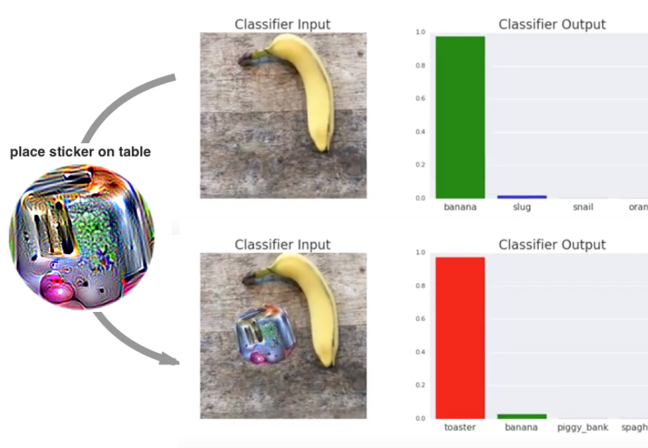
\includegraphics[width=\linewidth]{adversarial_patch.png}
    \caption{adversarial patch}
    \label{fig:patch}
\end{figure}
\cite{patch} In questo attacco si genera una patch che, quando entra nel campo visivo di un classificatore, causa un'errore di misclassificazione. Lo sviluppo dell'attacco è 
indipendente dalla immagine su cui viene generata. La patch generata può essere applicata direttamente alle immagini ma l'utilizzo più interessante è senza dubbio la stampa e l'applicazione di tale patch
ad oggetti fisici. In questo caso la patch potrebbe essere distribuita attraverso internet, stampata, e utiilizzata da un qualsiasi attaccante. Questo attacco è profondamente atipico rispetto
ai normali evasion attacks. La perturbazione è infatti di grandi dimensioni e questo potrebbe sembrare controintuitivo rispetto a ciò che sappiamo di tali attacchi. Ma il vantaggio principale
sta proprio nella sua natura unica. Una grande perturbazione è "resistente" anche rispetto ai normali metodi di difesa che si concentrano sulle piccole perturbazioni, ma che possono essere annullate in 
casi così estremi.
\subsection{Spatial Transformation}
\begin{figure}[h]
    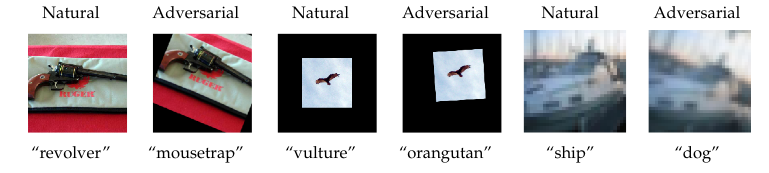
\includegraphics[width = \linewidth]{spat.png}
    \caption{esempi di trasformazioni avversarie}
    \label{fig:spat}
\end{figure}
\cite{spatial}La perturbazione generata è di tipo spaziale. Si cercano i parametri $(\delta u,\delta v,\theta)$ per cui un'immagine ruotata di un angolo $\theta$ e traslata di 
$(\delta u, \delta v)$ pixel viene classificata in modo errato, massimizzando la loss function. Questo tipo di perturbazioni può essere generato in modo "maligno", ma può anche essere causato da perturbazioni naturali(gli oggetti reali
non sempre appaiono perfettamente centrati).
\subsection{HopSkipJump}
\begin{figure}[h]
    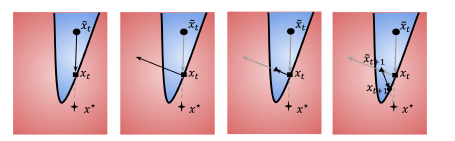
\includegraphics[width=\linewidth]{hop.png}
    \caption{funzionamento dell'hopskipjump}
    \label{fig:hop}
\end{figure}
È un attacco blackbox e necessita solo delle classi di output del modello. Parte da una grande perturbazione e punta a ridurla al minimo mantenendo comunque l'errore di classificazione.
La perturbazione viene ridotta attraverso diverse iterazioni di ricerca binaria. Ciascuna iterazione individua una nuova perturbazione valida, più "piccola" della precedente.
